\section{Otimização}\label{sec:otimizacao}

Historicamente, a otimização estrutural é classificada em três categorias conforme a natureza das variáveis de projeto manipuladas: otimização de seção (\textit{sizing}), otimização de forma (\textit{shape}) e otimização topológica (\textit{topology}) \parencite{BendsoeSigmund2003}.
Na otimização de seção, tanto a topologia quanto o contorno geométrico da estrutura permanecem fixos, e as variáveis de projeto correspondem a grandezas dimensionais dos elementos, como a área da seção transversal de barras ou a espessura de placas, conforme ilustrado na Figura~\ref{fig:tipos_otimizacao}a.
Na otimização de forma, a topologia também é mantida, porém a geometria do contorno do domínio é livre para variar, deslocando nós ou modificando a fronteira externa e interna da peça (Figura~\ref{fig:tipos_otimizacao}b).
Já a otimização topológica é a mais geral das três abordagens: nenhuma hipótese prévia é feita sobre a conectividade do material, o que permite o surgimento ou a eliminação de vazios internos e, consequentemente, a alteração da própria topologia da estrutura ao longo do processo de busca (Figura~\ref{fig:tipos_otimizacao}c).

\begin{figure}[htpb!]
\centering
\begin{tikzpicture}[
  support/.style={fill=black},
  member/.style={line cap=round},
  load/.style={-{Latex[length=2.2mm]}, thick},
  every node/.style={font=\footnotesize}
]

% ============ PAINEL A: OTIMIZACAO DE SECAO ============
\begin{scope}[xshift=0cm]
  \begin{scope}[yshift=2.6cm]
    \draw[member, line width=0.8pt] (0,0) -- (1,1);
    \draw[member, line width=0.8pt] (1,1) -- (2,0);
    \draw[member, line width=0.8pt] (0,0) -- (2,0);
    \draw[load] (1,1) -- (1,0.35);
    \filldraw (0,0) circle (2pt);
    \filldraw (2,0) circle (2pt);
    \draw (-0.15,-0.15) -- (0.15,-0.15) -- (0,0) -- cycle;
    \foreach \x in {-0.2,-0.05,0.1} \draw (\x,-0.15) -- (\x-0.12,-0.3);
    \draw[fill=white] (1.85,-0.15) circle (0.08);
    \draw (1.7,-0.23) -- (2.15,-0.23);
    \foreach \x in {1.75,1.9,2.05} \draw (\x,-0.23) -- (\x-0.12,-0.38);
  \end{scope}

  \draw[member, line width=2.6pt] (0,0) -- (1,1);
  \draw[member, line width=1pt]   (1,1) -- (2,0);
  \draw[member, line width=1.6pt] (0,0) -- (2,0);
  \draw[load] (1,1) -- (1,0.35);
  \filldraw (0,0) circle (2pt);
  \filldraw (2,0) circle (2pt);
  \draw (-0.15,-0.15) -- (0.15,-0.15) -- (0,0) -- cycle;
  \foreach \x in {-0.2,-0.05,0.1} \draw (\x,-0.15) -- (\x-0.12,-0.3);
  \draw[fill=white] (1.85,-0.15) circle (0.08);
  \draw (1.7,-0.23) -- (2.15,-0.23);
  \foreach \x in {1.75,1.9,2.05} \draw (\x,-0.23) -- (\x-0.12,-0.38);

  \draw[-{Latex[length=2.8mm]}, line width=0.9pt] (1,2.15) -- (1,1.15);
  \node[align=center] at (1,-1.0) {(a) Otimização de seção\\\textit{(sizing)}};
\end{scope}

% ============ PAINEL B: OTIMIZACAO DE FORMA ============
\begin{scope}[xshift=4.6cm]
  \begin{scope}[yshift=2.6cm]
    \draw[member, line width=1.2pt] (0,0) -- (1,0.7) -- (2,0) -- cycle;
    \draw[load] (1,0.7) -- (1,0.1);
    \filldraw (0,0) circle (2pt);
    \filldraw (2,0) circle (2pt);
    \draw (-0.15,-0.15) -- (0.15,-0.15) -- (0,0) -- cycle;
    \foreach \x in {-0.2,-0.05,0.1} \draw (\x,-0.15) -- (\x-0.12,-0.3);
    \draw[fill=white] (1.85,-0.15) circle (0.08);
    \draw (1.7,-0.23) -- (2.15,-0.23);
    \foreach \x in {1.75,1.9,2.05} \draw (\x,-0.23) -- (\x-0.12,-0.38);
  \end{scope}

  \draw[member, line width=1.2pt] (0,0) -- (1.35,1.15) -- (2,0) -- cycle;
  \draw[load] (1.35,1.15) -- (1.35,0.55);
  \filldraw (0,0) circle (2pt);
  \filldraw (2,0) circle (2pt);
  \draw (-0.15,-0.15) -- (0.15,-0.15) -- (0,0) -- cycle;
  \foreach \x in {-0.2,-0.05,0.1} \draw (\x,-0.15) -- (\x-0.12,-0.3);
  \draw[fill=white] (1.85,-0.15) circle (0.08);
  \draw (1.7,-0.23) -- (2.15,-0.23);
  \foreach \x in {1.75,1.9,2.05} \draw (\x,-0.23) -- (\x-0.12,-0.38);

  \draw[-{Latex[length=2.8mm]}, line width=0.9pt] (1,2.15) -- (1,1.15);
  \node[align=center] at (1,-1.0) {(b) Otimização de forma\\\textit{(shape)}};
\end{scope}

% ============ PAINEL C: OTIMIZACAO TOPOLOGICA ============
\begin{scope}[xshift=9.2cm]
  \begin{scope}[yshift=2.6cm]
    \fill[pattern=north east lines, pattern color=black!55] (0,0) rectangle (2,1);
    \draw (0,0) rectangle (2,1);
    \draw[load] (2,0.5) -- (2.65,0.5);
    \draw (-0.15,0) -- (-0.15,1);
    \foreach \y in {0,0.25,0.5,0.75,1} \draw (-0.15,\y) -- (-0.3,\y-0.15);
  \end{scope}

  \draw (0,0) rectangle (2,1);
  \draw[member, line width=1.1pt] (0,0) -- (2,1);
  \draw[member, line width=1.1pt] (0,1) -- (2,0);
  \draw[load] (2,0.5) -- (2.65,0.5);
  \draw (-0.15,0) -- (-0.15,1);
  \foreach \y in {0,0.25,0.5,0.75,1} \draw (-0.15,\y) -- (-0.3,\y-0.15);

  \draw[-{Latex[length=2.8mm]}, line width=0.9pt] (1,2.15) -- (1,1.15);
  \node[align=center] at (1,-1.0) {(c) Otimização topológica\\\textit{(topology)}};
\end{scope}

\end{tikzpicture}
\caption{Classificação clássica da otimização estrutural conforme a natureza das variáveis de projeto: (a) seção; (b) forma; (c) topológica.}
\label{fig:tipos_otimizacao}
\end{figure}

Este trabalho situa-se na primeira categoria: o dimensionamento das longarinas e das pranchas do tabuleiro é tratado como um problema de otimização de seção, no qual a topologia do sistema estrutural -- número e disposição das peças -- é definida \textit{a priori} pelo projetista, e o algoritmo busca as dimensões ótimas dessas peças dentro dos limites estabelecidos.

\subsection{Histórico da otimização de pontes}\label{sec:historico_otimizacao_pontes}

A aplicação de técnicas de otimização ao projeto de pontes antecede a difusão dos algoritmos evolutivos.
Na década de 1970, \textcite{Aguilar1973} apresentaram um procedimento computacional baseado em programação dinâmica para selecionar configurações econômicas de pontes rodoviárias com múltiplos vãos simplesmente apoiados.
O modelo permitia investigar conjuntamente a geometria, as condições do terreno, os custos de construção e a escolha do número, do comprimento e do tipo dos vãos.
Posteriormente, \textcite{Brar1984} empregaram programação geométrica na solução de dois problemas de projeto de pontes, comparando o custo de uma das soluções obtidas com o de um projeto usual.
Esses trabalhos exemplificam uma orientação inicial para a redução de custos por meio da exploração sistemática de alternativas que, no procedimento convencional, dependiam principalmente da experiência do projetista.

Na década de 1990, essa abordagem foi ampliada para considerar diferentes níveis de decisão e múltiplos critérios de desempenho.
\textcite{CohnLounis1994} organizaram o projeto ótimo de superestruturas de pontes de concreto em três níveis: otimização dos componentes, da configuração estrutural e do sistema global.
Os autores consideraram, separada ou simultaneamente, objetivos associados ao custo, ao consumo de concreto e de aço de protensão e à altura da superestrutura, combinando programação não linear e procedimentos de busca.
O estudo evidencia que a otimização de uma seção isolada não substitui a avaliação da configuração da ponte como um todo, pois as escolhas de tipologia e de distribuição dos vãos também interferem na solução econômica.

Em paralelo, a otimização de pontes metálicas estaiadas incorporou a interação entre dimensões das peças, geometria e distribuição dos esforços.
\textcite{SimoesNegrao1994} formularam um problema multiobjetivo com metas de redução de custo e de tensões, adotando como variáveis as dimensões das seções e as posições de ancoragem dos estais no tabuleiro e nas torres.
O procedimento, baseado em um algoritmo de otimização por entropia, também examinou a influência das tensões decorrentes da sequência construtiva.
Assim, a literatura já contemplava soluções de compromisso e variáveis de forma antes da popularização das metaheurísticas multiobjetivo atualmente empregadas.

Uma vertente posterior passou a explorar metaheurísticas para tratar problemas com numerosas variáveis discretas e verificações estruturais acopladas.
\textcite{Marti2013} aplicaram uma estratégia híbrida de recozimento simulado com operador de mutação ao projeto de pontes rodoviárias com vigas pré-moldadas e protendidas de seção em U.
O problema compreendia 59 variáveis discretas, relacionadas à geometria, aos materiais e às armaduras, e buscava minimizar custos de fabricação, transporte e construção, respeitando as verificações dos estados limites.
Essa aplicação ilustra a possibilidade de incorporar decisões construtivas ao processo de busca e de produzir relações paramétricas úteis ao projeto de pontes.

A ampliação dos critérios de projeto também levou à consideração conjunta de aspectos econômicos, ambientais e de segurança.
\textcite{GarciaSeguraYepes2016} empregaram busca harmônica multiobjetivo no projeto de pontes rodoviárias de concreto pós-tensionado com seção caixão, minimizando o custo e as emissões de CO\textsubscript{2} e maximizando um fator global de segurança.
Nesse caso, a análise por elementos finitos e a verificação dos estados limites foram integradas à busca de soluções de Pareto.
Em seguida, \textcite{GarciaSegura2017} estenderam a investigação ao desempenho ao longo da vida útil de pontes sujeitas à corrosão, articulando alternativas de projeto inicial e estratégias de manutenção sob uma meta de confiabilidade.
Esses estudos mostram como a avaliação das soluções pode ultrapassar o custo inicial e incluir consequências ambientais e a evolução da segurança estrutural no tempo.

Mais recentemente, a integração entre otimização e modelagem paramétrica passou a permitir a atualização automática da geometria, da análise e das verificações de projeto.
\textcite{deMoraes2025} combinaram modelagem tridimensional, algoritmo genético, análise por elementos finitos e busca local pelo método Simplex no projeto de pontes com vigas de concreto protendido.
A abordagem relaciona decisões sobre a configuração global da ponte ao dimensionamento de suas vigas, aproximando a otimização das etapas de elaboração e avaliação do modelo estrutural.

No caso da madeira, há antecedentes específicos de otimização de passarelas estaiadas.
\textcite{Negrao1999} investigou a minimização de custo mediante a alteração das dimensões dos elementos, das características dos estais e de parâmetros geométricos, incluindo a escolha de propriedades associadas às classes de madeira laminada colada.
Posteriormente, \textcite{SimoesNegrao2005} apresentaram um procedimento de projeto ótimo baseado em confiabilidade para passarelas estaiadas de madeira laminada colada, integrando análise por elementos finitos, análise de sensibilidade e uma formulação multicritério que considera custo, tensões, deslocamentos e confiabilidade.
Esses antecedentes demonstram que tanto a busca de soluções econômicas quanto a consideração de incertezas já fazem parte da pesquisa sobre pontes de madeira, embora em sistemas estruturais distintos das pontes rodoviárias de madeira roliça estudadas neste trabalho.

O conjunto desses trabalhos permite identificar uma ampliação das decisões e dos critérios incorporados à otimização de pontes: da busca de configurações de menor custo às formulações que articulam desempenho estrutural, impactos ambientais, confiabilidade e automação do projeto.
Nesse contexto, o presente estudo concentra-se no dimensionamento das seções de longarinas de madeira roliça e de pranchas do tabuleiro, com uma formulação multiobjetivo e avaliação de perturbações dimensionais.
Esse tratamento de robustez, detalhado na Seção~\ref{sec:robustez}, avalia a resposta das soluções às variações prescritas nas dimensões; ele não corresponde, por si só, à imposição de uma probabilidade de falha ou de um índice-alvo de confiabilidade.
A formulação multiobjetivo utilizada é apresentada a seguir.

\subsection{Estrutura de otimização multiobjetivo}\label{sec:otim_multiobjetivo}

Um problema de otimização multiobjetivo envolve a minimização e/ou maximização simultânea de múltiplas funções objetivo, sujeitas a um conjunto de restrições que definem a viabilidade das soluções candidatas.
Diferentemente da otimização monoobjetivo, essa formulação não conduz a uma única solução ótima global.
Alternativamente, resulta em um conjunto de soluções ótimas de Pareto, cada uma representando um caso distinto de compromisso (\textit{trade-off}) entre critérios de desempenho concorrentes.
 
A formulação matemática geral de um problema de otimização multiobjetivo pode ser expressa conforme a Equação~\eqref{eq:mop}.
 
\begin{equation}
\left\{
\begin{array}{ll}
f_m(\mathbf{x}), & m = 1,2,\ldots,M; \\
g_j(\mathbf{x}) \leq 0, & j = 1,2,\ldots,J; \\
h_k(\mathbf{x}) = 0, & k = 1,2,\ldots,K; \\
x_i^{(L)} \leq x_i \leq x_i^{(U)}, & i = 1,2,\ldots,n.
\end{array}
\right.
\label{eq:mop}
\end{equation}
 
 Nesta formulação, o vetor de funções objetivo é definido segundo a Equação
 ~\eqref{eq:fx}.
 
 \begin{equation}
 f(\mathbf{x}) = \left(f_1(\mathbf{x}), f_2(\mathbf{x}), \ldots, f_M(\mathbf{x})\right)^T\label{eq:fx}
 \end{equation}
 
 Onde $\mathbf{x} = (x_1, x_2, \ldots, x_n)^T$ 
representa o vetor $n$-dimensional de variáveis de projeto.
O espaço de projeto viável é delimitado pelas restrições de desigualdade $g_j(\mathbf{x})$, restrições de igualdade $h_k(\mathbf{x})$ e restrições de domínio definidas pelos limites inferior $x_i^{(L)}$ e superior $x_i^{(U)}$, que em conjunto estabelecem o domínio admissível $(D)$ \parencite{DEB2009}.

Objetivos inicialmente concebidos como problemas de maximização são convertidos em problemas equivalentes de minimização mediante a multiplicação das respectivas funções objetivo por $-1$, garantindo uma estrutura computacional unificada.
A Figura~\ref{fig:pareto} ilustra o espaço de soluções de um problema biobjetivo típico, destacando a diversidade de configurações viáveis e o conceito de fronteira de Pareto.

 \begin{figure}[htpb!]
 \centering
 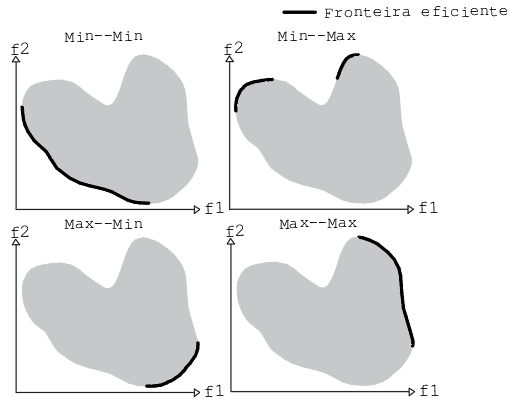
\includegraphics[width=0.6\textwidth]{figuras/z_types_frontier.png}
 \caption{Possíveis soluções de um problema de otimização multiobjetivo \parencite{DEB2009}.}
 \label{fig:pareto}
 \end{figure}
 
 \subsection{Algoritmo de otimização NSGA-II} \label{sec:nsga2}
 
 Desenvolvido por \textcite{DEB2009}, este algoritmo evolutivo consolidou-se na literatura por sua capacidade de aproximar de forma eficiente o conjunto ótimo de Pareto. 
O NSGA-II preserva a natureza vetorial do problema multiobjetivo e busca um conjunto diverso de soluções não dominadas, sem recorrer à escalarização (soma ponderada) das funções objetivo.
O mecanismo central do algoritmo baseia-se na classificação rápida de não dominância (\textit{Fast Non-Dominated Sorting}).
A cada geração iterativa, toda a população de indivíduos é avaliada e ordenada em frentes sucessivas de não dominância $\mathcal{F}_1, \mathcal{F}_2, \ldots, \mathcal{F}_k$.
A primeira frente ($\mathcal{F}_1$) agrupa as soluções temporariamente ótimas daquela geração, constituindo a aproximação corrente da fronteira de Pareto.
A frente subsequente ($\mathcal{F}_2$) abriga soluções que seriam dominantes caso os indivíduos da frente $\mathcal{F}_1$ fossem desconsiderados, e assim por diante.Para garantir que a busca não convirja prematuramente para uma única região e mantenha uma dispersão uniforme ao longo da fronteira, o algoritmo utiliza o operador de distância de aglomeração (\textit{crowding distance}).
Esta métrica estima a densidade de soluções em torno de um determinado indivíduo, calculando o hipervolume formado pelos seus vizinhos mais próximos.
Para um problema com $M$ funções objetivo, a distância de aglomeração $d_i$ do indivíduo $i$ é calculada conforme a Equação~\eqref{eq:crowding}.
 
 \begin{equation}d_i = \sum_{m=1}^{M} \frac{f_m(\mathbf{x}_{i+1}) - f_m(\mathbf{x}_{i-1})}{f_m^{\max} - f_m^{\min}}
 \label{eq:crowding}
 \end{equation}
 
O NSGA-II emprega uma estratégia fortemente elitista.
A cada ciclo, as populações parental e descendente são combinadas e ordenadas primeiramente pelo nível de Pareto e, em caso de empate na mesma frente, pela maior distância de aglomeração.
O Algoritmo~\ref{alg:nsga2} resume a lógica evolutiva e o fluxo de avaliações estruturais, incorporando a proteção contra incertezas descrita na Seção~\ref{sec:robustez}.
 
 \begin{algorithm}[!ht]
 \caption{Otimização robusta multiobjetivo via NSGA-II}
 \label{alg:nsga2}
 \begin{algorithmic}[1]
 \Require Limites $[x_i^{(L)}, x_i^{(U)}]$, tamanho da população $N_{pop}$, gerações $N_{gen}$, desvio de robustez $\rho$, número de checagens $N_c$
 \Ensure Fronteira eficiente $\mathcal{F}_1$
 \State Inicializar população $P_0$ por amostragem aleatória em $[x_i^{(L)}, x_i^{(U)}]$
 \For{cada geração $t = 0$ até $N_{gen}-1$}
   \For{cada indivíduo $\mathbf{x} \in P_t$}
     \State $\mathbf{F} \gets \mathbf{0}$;\ $\mathbf{G} \gets \mathbf{0}$
     \For{$c = 1$ até $N_c$} \Comment{avaliação estocástica}
       \State $\tilde{\mathbf{x}} \gets \mathbf{x}\,(1 + \rho\,\boldsymbol{\xi})$, com $\boldsymbol{\xi} \sim \mathcal{U}(-1,1)$
       \State $(\mathbf{f}, \mathbf{g}) \gets$ \Call{AvaliarModelo}{$\tilde{\mathbf{x}}$}
       \State $\mathbf{F} \gets \mathbf{F} + \mathbf{f}$;\ $\mathbf{G} \gets \mathbf{G} + \mathbf{g}$
     \EndFor
     \State $\mathbf{F} \gets \mathbf{F}/N_c$;\ $\mathbf{G} \gets \mathbf{G}/N_c$ \Comment{agregação estatística}
   \EndFor
   \State $Q_t \gets$ seleção por torneio, cruzamento SBX e mutação polinomial sobre $P_t$
   \State $R_t \gets P_t \cup Q_t$
   \State Ordenar $R_t$ em frentes não dominadas $\{\mathcal{F}_1, \mathcal{F}_2, \ldots\}$
   \State $P_{t+1} \gets$ melhores $N_{pop}$ indivíduos por nível de Pareto e distância de aglomeração
 \EndFor
 \State \Return $\mathcal{F}_1$
 \end{algorithmic}
 \end{algorithm}

Para a evolução das gerações, o algoritmo baseia-se em operadores genéticos específicos para o tratamento de variáveis contínuas.
A aplicação conjunta do cruzamento simulado binário (SBX) e da mutação polinomial (PM) permite refinar as soluções locais no espaço de busca, ao passo que a eliminação sistemática de duplicatas resguarda a diversidade genética da população, prevenindo a convergência prematura.
Os parâmetros de configuração adotados em todas as execuções deste trabalho estão reunidos na Tabela~\ref{tab:nsga2}.

\begin{table}[!ht]
\caption{Parâmetros de configuração do NSGA-II.\label{tab:nsga2}}
\begin{tabular*}{\columnwidth}{@{\extracolsep\fill}lc@{\extracolsep\fill}}
\toprule
Parâmetro & Valor \\
\midrule
Tamanho da população, $N_{pop}$ & 50 \\
Número de gerações, $N_{gen}$ & 150 \\
Amostragem inicial & Aleatória uniforme \\
Cruzamento & SBX, $p_c = 0{,}90$, $\eta_c = 15$ \\
Mutação & Polinomial, $\eta_m = 20$ \\
Eliminação de duplicatas & Sim \\
Semente aleatória & 1 \\
Número de checagens robustas, $N_c$ & 30 \\
Desvio de robustez, $\rho$ & 5\% \\
\bottomrule
\end{tabular*}
\end{table}
 
 \subsection{Robustez na otimização}\label{sec:robustez}
 
Na engenharia estrutural, a otimização puramente determinística tende a posicionar as soluções ótimas exatamente sobre a fronteira matemática das restrições ativas.
Essa característica as torna extremamente sensíveis a pequenas variações nas variáveis de projeto.
Na prática, essa sensibilidade é agravada pela variabilidade inerente às propriedades físicas dos materiais empregados e pelas tolerâncias naturais de fabricação, corte e montagem das peças.
Sob condições reais, uma estrutura cujo projeto encontre-se no limite exato de viabilidade determinística possui alta probabilidade de violar normas de segurança ou estados limites de serviço caso suas dimensões finais desviem minimamente do previsto.
Para mitigar esse efeito, o conceito de robustez deve ser incorporado de forma nativa ao processo algorítmico.
A estratégia adotada para inserir robustez na otimização consiste em avaliar cada solução candidata não apenas em seus valores nominais de projeto, mas também sob a influência de um conjunto de perturbações estatísticas controladas.
Para um dado indivíduo $\mathbf{x}$, são geradas $N_c$ realizações perturbadas, denotadas por $\tilde{\mathbf{x}}^{(c)}$, conforme definido na Equação~\eqref{eq:perturbacao}.
 
 \begin{equation}\tilde{x}_i^{(c)} = x_i \left(1 + \rho\,\xi_i^{(c)}\right),\qquad \xi_i^{(c)} \sim \mathcal{U}(-1,\,1)\label{eq:perturbacao}
 \end{equation}
 
O termo $\rho$ representa a magnitude do desvio paramétrico tolerado pelo projeto em relação ao valor nominal, e $\xi_i^{(c)}$ descreve uma variável aleatória com distribuição de probabilidade uniforme no intervalo de $[-1, 1]$.
Em cada ciclo, as avaliações perturbadas são processadas independentemente no modelo analítico.
Posteriormente, as funções objetivo e os valores das restrições são agregados por meio do operador de esperança matemática (média simples), de acordo com as Equações~\eqref{eq:fmed} e~\eqref{eq:gmed}.
 
 \begin{equation}\bar{f}_m(\mathbf{x}) = \frac{1}{N_c}\sum_{c=1}^{N_c} f_m\!\left(\tilde{\mathbf{x}}^{(c)}\right)
 \label{eq:fmed}
 \end{equation}

 \begin{equation}\bar{g}_j(\mathbf{x}) = \frac{1}{N_c}\sum_{c=1}^{N_c} g_j\!\left(\tilde{\mathbf{x}}^{(c)}\right)
 \label{eq:gmed}
 \end{equation}
 
Por meio desta formulação, uma solução só é julgada admissível se suas restrições médias permanecerem viáveis ($\bar{g}_j \leq 0$) mesmo sob a oscilação aleatória dos parâmetros: projetos configurados muito próximos das restrições acumulam violações durante o sorteio das perturbações desfavoráveis, inflacionando $\bar{g}_j$ e sendo penalizados pelo mecanismo de viabilidade do algoritmo.
O resultado é o deslocamento natural da fronteira de Pareto rumo a zonas mais conservadoras do espaço viável de projeto.
